\chapter{Introduzione}

Fin dai primi anni del XX secolo, con la nascita dell'industria automobilistica, i produttori di automobili hanno cercato di migliorare i sistemi di sicurezza installati all'interno dei veicoli, ovviamente tutto in funzione di quanto la tecnologia potesse offrire al momento. Si è partiti, ad esempio, dall'introduzione dei freni a disco, per poi passare alle cinture di sicurezza, alla disponibilità degli airbag e all'introduzione dei primi sistemi quali ABS e simili. Ogni nuova tecnologia ha richiesto anni di ricerca e test prima di essere rilasciata e diventare uno standard per i nuovi modelli.

Nell'ultimo ventennio, con l'obiettivo di aumentare la sicurezza dei veicoli, sono stati compiuti notevoli sforzi nel campo degli \textit{Intelligent Transport System (ITS)}, anche alla luce di quanto definito dalla direttiva 2010/40/EU dell'Unione Europea \cite{2010-40}. Questo paradigma comprende una serie di applicazioni e servizi utili non solo per la sicurezza del conducente e dei passeggeri, ma anche per la loro esperienza di guida, per l'efficienza del traffico e diverse altre esigenze di trasporto. Le applicazioni legate alla sicurezza e all'efficienza sono interconnesse e si avvantaggiano reciprocamente, motivo per cui l'industria automobilistica, enti governativi e numerosi ricercatori accademici collaborano per standardizzare tutti gli aspetti dei sistemi ITS.

I progressi verso la realizzazione dei sistemi ITS sono stati alimentati da importanti sviluppi nelle \textit{Vehicular Ad-hoc NETworks (VANET)}. Questa tecnologia è stata fondamentale per il successo dei sistemi ITS, consentendo uno scambio rapido e diretto di informazioni necessarie per la maggior parte delle applicazioni ITS. L'introduzione delle VANET, attraverso l'uso della \textit{Dedicated Short-Range Communication (DSRC)}, ha reso possibile lo scambio di messaggi tra \textit{Vehicle-to-Vehicle (V2V)} e \textit{Vehicle-to-Infrastructure (V2I)}.

Uno dei punti cardine, nell'implementazione delle comunicazioni V2V e V2I, è stato quello della standardizzazione, da parte di ETSI, dei cosiddetti \textit{Cooperative Awareness Messages (CAMs)} che trova la sua applicazione principale nelle applicazioni deputate alla \textit{Collision Avoidance}, ovvero tutti gli strumenti applicativi atti a prevenire tutta una serie di situazioni di pericolo tra i vari veicoli e tutto ciò che può essere presente sulla sede stradale.

Le CA beneficiano dell'aumento del numero di sensori e della potenza di calcolo presenti nei veicoli moderni, che hanno già portato a funzionalità innovative come la Frenata Automatica d'Emergenza. Tuttavia, queste capacità sono limitate a una visione locale del veicolo; l'idea è di ampliare questa visione condividendo informazioni tramite le VANET con altri veicoli e unità stradali, con l'obiettivo di abilitare applicazioni sempre più complesse ed efficaci. 
Questo porta implicitamente alla creazione di una rete composta da nodi, rappresentati da veicoli e infrastrutture stradali, che presenta una serie di sfide sia implementative che prestazionali. Questi problemi richiedono approcci specifici e soluzioni diverse rispetto a quelle adottate nelle reti tradizionali, poiché le condizioni operative e i vincoli presenti sono completamente diversi \cite{risma2021implementation}.

\section{VANET}
Una \textit{VANET (Vehicular Ad-hoc Network)} è una classe distintiva di \textit{MANET (Mobile Ad-hoc Network)} in cui i veicoli in movimento fungono da nodi o router per scambiare messaggi tra di loro, o come \textit{Access Point (AP)}. Solitamente, una VANET può connettere veicoli entro un raggio di circa 1 chilometro al massimo utilizzando lo standard IEEE 802.11p. Il suo obiettivo è supportare sia la comunicazione \textit{Vehicle-to-Vehicular (V2V)} che \textit{Vehicle-to-Infrastructure (V2I)} in una rete senza infrastruttura. Sono state avviate numerose iniziative di ricerca, in Europa, negli Stati Uniti e in Giappone, per rendere gli ITS una realtà; alcune di queste sono \textit{COOPERS, CVIS, SAFESPOT, PReVENT}, \textit{Advanced Safety Vehicle Program (ASV)} ed infine \textit{Wireless Access in Vehicular Environments (WAVE)}, su cui si baserà in parte il lavoro descritto in questo elaborato.

Le VANET vengono utilizzate per supportare applicazioni critiche per la sicurezza e applicazioni di intrattenimento non legate alla sicurezza. Le applicazioni di sicurezza, come l'evitamento delle collisioni, la rilevazione pre-collisione o il cambio di corsia, mirano a ridurre gli incidenti stradali attraverso il monitoraggio e la gestione del traffico. Le applicazioni non di sicurezza consentono ai passeggeri di accedere a vari servizi come internet, comunicazione interattiva, giochi online, servizi di pagamento e aggiornamenti informativi mentre i veicoli sono in movimento. La principale differenza tra le applicazioni di sicurezza e quelle non di sicurezza è che le prime sono in grado di inviare e elaborare messaggi in tempo reale. Sia i conducenti che i passeggeri possono accedere a entrambi i tipi di servizi dall'infrastruttura vicina in modo fluido utilizzando tecnologie di accesso wireless.

Le VANET e le MANET condividono molte somiglianze, come la topologia dinamica, la trasmissione dati multi-hop, l'architettura distribuita e la trasmissione omnidirezionale. In entrambe le reti, i nodi mobili possono instradare o rilanciare dati verso la destinazione autonomamente. Tuttavia, ci sono alcune differenze significative tra VANET e MANET. Poiché i veicoli si muovono lungo la strada, la mobilità dei nodi in una VANET è prevedibile, a differenza di una MANET. Inoltre, non ci sono limitazioni in termini di capacità di archiviazione, potenza di elaborazione e durata della batteria dei nodi in una VANET. A causa del rapido movimento dei nodi, la topologia della rete wireless formata è altamente dinamica (Figura \ref{fig:vanet}). Inoltre, la densità della rete in una VANET varia significativamente nel tempo e nello spazio \cite{anwer2014survey} \cite{vehicular-ad-hoc}.

\begin{figure}[h!]
    \centering
    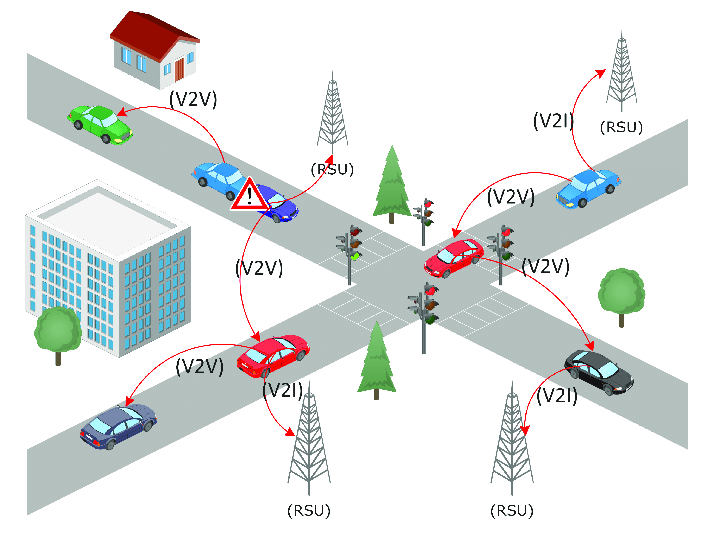
\includegraphics[width=0.7\textwidth]{vanet.png}
    \caption{VANET}
    \label{fig:vanet}
\end{figure}

Tipicamente, una VANET è composta da tre componenti principali (Figura \ref{fig:obu_rsu}): 
\begin{itemize}
    \item \textbf{On Board Unit (OBU)}: dispositivo embedded inserito all'interno di ogni veicolo comunicante con gli altri mediante un'interfaccia Wireless.
    \item \textbf{Road Side Unit (RSU)}: dispositivo fisso in genere posizionato ai lati della strada; funge da intermediario tra le \textit{On Board Unit} dei veicoli e le infrastrutture stradali e la rete Internet.
    \item \textbf{GNSS}: sistema di geolocalizzazione tipo \textit{GPS (Global Positioning System), GLONASS (GLObal NAvigation Satellite System) o Galileo}.
\end{itemize}

\begin{figure}[h!]
    \centering
    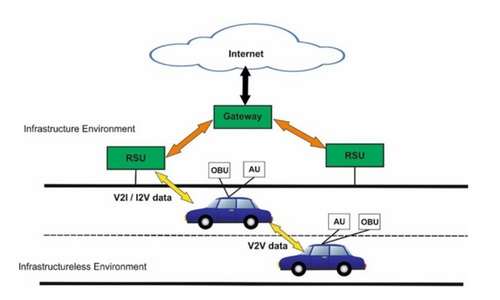
\includegraphics[width=1\textwidth]{routing_vanet.jpeg}
    \caption{OBU e RSU}
    \label{fig:obu_rsu}
\end{figure}

Tutti questi componenti comunicano utilizzando standard/protocolli di comunicazione wireless che determinano vari aspetti della comunicazione, come raggio e velocità di trasmissione dei dati, latenza e sicurezza. La consegna dei dati è considerata una delle sfide principali a causa dei rapidi cambiamenti di topologia, delle frequenti interruzioni del segnale e delle opportunità di contatto nelle VANET. 

\section{Obiettivi}
L'obiettivo principale di questo lavoro sarà lo studio e la realizzazione di un algoritmo DCC (\textit{Decentralized Congestion Control}) in un ambiente Linux per dispositivi che supportano lo standard IEEE 802.11p. Esso verrà svolto mediante la configurazione di un test bed apposito, composto da quattro dispositivi Rock, che verrà descritto successivamente.

Uno degli aspetti critici delle VANET è la gestione della congestione, che può compromettere le prestazioni della rete e, di conseguenza, l'efficacia delle applicazioni di sicurezza e infotainment. In questo contesto, il \textit{Decentralized Congestion Control (DCC)} emerge come una soluzione fondamentale. Il DCC consente ai veicoli di gestire la congestione in modo autonomo, senza la necessità di un controllo centralizzato, regolando dinamicamente il flusso di dati, ottimizzando l'uso delle risorse di rete e garantendo una trasmissione più fluida delle informazioni.

Ci si propone, quindi, di analizzare in dettaglio i protocolli IEEE 802.11p e DCC, esaminando le loro caratteristiche tecniche e il loro funzionamento nel contesto delle VANET, con particolare riferimento agli standard \textit{ETSI (European Telecommunications Standards Institute)}. Attraverso un'analisi delle performance su piattaforme Linux, si valuteranno l'efficacia dei protocolli in differenti scenari, considerando vari parametri di prestazione.

Un aspetto fondamentale di questa ricerca sarà, inoltre, l'integrazione delle metriche di \textit{Quality of Service (QoS)} utilizzando strumenti come iPerf. Questa integrazione permetterà di misurare e ottimizzare le prestazioni della rete, fornendo dati preziosi su throughput e variabilità di esso, che sono essenziali al fine di garantire un'esperienza utente ottimale soprattutto nelle applicazioni di sicurezza ma anche in quelle di infotainment.